
\documentclass{article}
\usepackage{mathtools, amssymb, amsthm, graphicx, ulem} % imports amsmath
\usepackage[a4paper, margin=1in]{geometry} % Set margins for better layout
\begin{document}
\sloppy

\section{První příklad zadání C}

\begin{figure}[!ht]
  \centering
  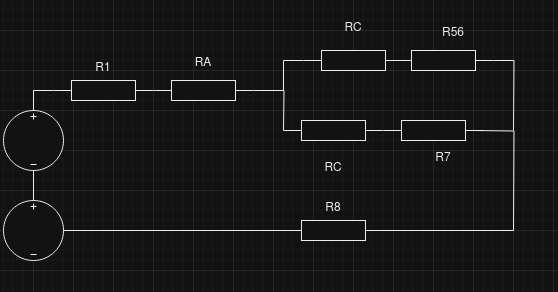
\includegraphics[width=0.9\textwidth, keepaspectratio]{/home/tjoslef/skola/zapisky/vut/IEL/projekt/uprava_hvezdu_1.png}
  \caption{Úprava pomocí hvězdy}
  \label{fig:hvezda}
\end{figure}

\[
    R_{56} = \frac{R_6 \times R_5}{R_6 + R_5}
\]

\begin{figure}[!ht]
  \centering
  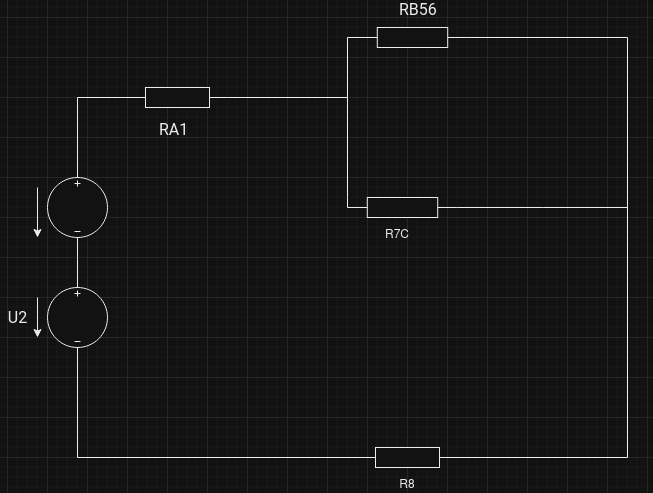
\includegraphics[width=0.9\textwidth, keepaspectratio]{/home/tjoslef/skola/zapisky/vut/IEL/projekt/dalsi uprava.png}
  \caption{Další úprava}
  \label{fig:dalsi_uprava}
\end{figure}

\[
R_{A1} = \frac{R_2 \times R_3}{R_2 + R_3 + R_4} + R_1
\]
\[
    R_{A1} = \frac{810 \times 220}{810 + 220 + 190} + 450 \quad \Rightarrow \quad R_{41} = 596.066
\]

\[
R_{B56} = \frac{R_2 \times R_4}{R_2 + R_3 + R_4} + \frac{R_6 \times R_5}{R_6 + R_5}
\]
\[
R_{B56} = \frac{810 \times 220}{810 + 190 + 720} + \frac{220 \times 720}{220 + 720}
= 272.115
\]
\[
R_{C7} = \frac{R_3 \times R_4}{R_2 + R_3 + R_4} + R_7
\]
\[
R_{C7} = \frac{190 \times 220}{810 + 190 + 720} + 260 = 284.302
\]

\[
R  = \frac{272.115 \times 284.320}{272.115 + 284.320} + 596.066 + 180 \quad \Rightarrow \quad R = 915.107
\]

\[
I = \frac{U}{R} = \frac{180}{894.770} \quad \Rightarrow \quad I = 0.1967
\]

\[
    U_{R3} = U - U_{R7} - U_{R1}
\]
\[
U_{R7} = R_7 \times I
\]
\[
    U_{R1} = R_1 \times I
\]
\[
U_{R7} = 260 \times 0.1967 = 51.114 \, \text{V}
\]
\[
    U_{R1} = 450 \times 0.1967 = 88.515 \, \text{V}
\]
\[
U_{R3}  = 180 - 51.114 - 88.515 = 40.371 \, \text{V}
\]

\[
I_{R3} = \frac{U_{R3}}{R_3}
\]
\[
I_{R3} = \frac{40.371}{190} = 0.212 \, \text{A}
\]

\clearpage
\section{Reseni druheho prikladu}

\[
    \text{Uzel A:} \quad \frac{130 - U_A}{47} + \frac{U_A - U_B}{28} - \frac{90 - (U_A - U_B)}{58} - \frac{U_A}{39} = 0
\]
\[
    \text{Uzel B:} \quad \frac{5}{10} + \frac{90 - (U_A - U_B)}{58} - \frac{U_A - U_B}{28} - \frac{U_C - U_B}{35} = 0
\]
\[
    \text{Uzel C:} \quad \frac{U_C - U_B}{35} - \frac{5}{10} - \frac{U_C}{25} = 0
\]
\begin{align}
    8987U_A - 78819U_B &= -1807260 \\
    -215U_A + 331U_B - 116U_C &= -8330 \\
    -10U_B - 4U_C &= 175
\end{align}
\section{Řešení třetího příkladu}
Úprava:

\begin{figure}[!ht]
  \centering
  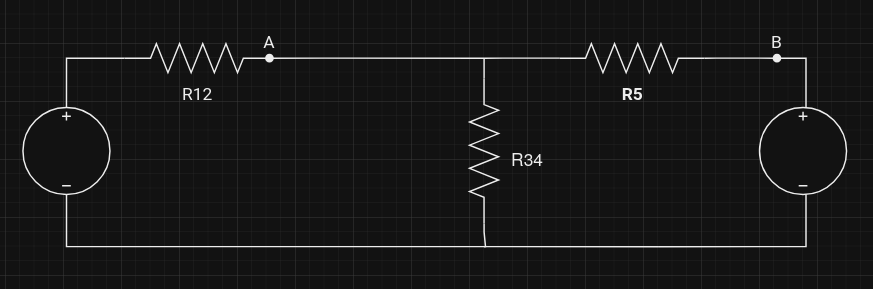
\includegraphics[width=0.9\textwidth, keepaspectratio]{/home/tjoslef/skola/zapisky/vut/IEL/projekt/uprava_priklad3.png}
  \caption{Další úprava}
  \label{fig:upravapriklad3}
\end{figure}

\[
    R_i = \frac{R_{12} \times R_5}{R_{12} + R_5}
\]
\[
    R_i = \frac{950 \times 80}{950 + 80} \quad \Rightarrow \quad R_i = 73.786
\]
\[
    I_x = \frac{U_2 - U_1}{R_{12} + R_5}
\]
\[
    I_x = \frac{180 - 130}{950 + 80} \quad \Rightarrow \quad I_x = 0.049
\]
\[
    U_i = U_1 + R_i \times I_x
\]
\[
    U_i = 130 + 950 \times 0.049
\]
\[
    I_{R34} = \frac{U_i}{R_i + R_{34}}
\]
\[
    \frac{176.55}{73.786 + 150}
\]

\end{document}


